\documentclass[11pt,onecolumn]{article} 
\usepackage{latex8}
\bibliographystyle{latex8}
%\usepackage{times}	
\usepackage{graphicx}
\usepackage[top=2.5cm, bottom=2.5cm, left=3cm, right=3cm]{geometry}
\usepackage[font={small}]{caption}
\usepackage{subcaption}


\begin{document}
%
% paper title
% can use linebreaks \\ within to get better formatting as desired
\title{Benchmarking Graph database/processing systems\\for Agglomerative Clustering}


% author names and affiliations
% use a multiple column layout for up to two different
% affiliations

\author{
 Ashish Jain\\
 \textit{ashishjain@cs.umass.edu}\\
School of Computer Science\\
University of Massachusetts Amherst\\
\and
 Vijay Pasikanti\\
 \textit{vijaykp@cs.umass.edu}\\
School of Computer Science\\
University of Massachusetts Amherst\\
\and
Gerome Miklau\\
\textit{miklau@cs.umass.edu}\\
School of Computer Science\\
University of Massachusetts Amherst\\
}
% make title
\maketitle

\begin{abstract}
Graph data is getting increasingly popular in, e.g. text processing, social networks etc. Over the years it lead to the development of various graph databases and graph processing system. A recent study by [1:??] benchmarks the graph and relational databases. However, according to our knowledge there has been no study on benchmarking the graph databases and graph processing systems to compare their effectiveness.  Therefore our proposal is novel in terms of task. In this paper we take one of the most expensive data mining technique i.e. clustering, to benchmark the two systems. Since personal social networks are big and cluttered, clustering is an effective technique to organize and find out community structure within the social network graphs. We are using Neo4j and GraphLab as our graph database and graph processing system respectively.
\end{abstract}


\textbf{Keywords:} Clustering, graph database, graph processing, Neo4j and GraphLab

\Section{Introduction}
There has been great deal of discussion recently on the subject of graph processing. With the explosion of social networks like Facebook, Twitter etc and other complex, inter-dependent datasets, graph storage and processing has emerged as one of the new computational challenges in the field of big data. Since the social data with connections between people provides a graph like structure to it, finding efficient ways to process it and discovering close-knit clusters in these networks is of fundamental interest to us.
\\\\
Currently, users in Facebook, Google+ and Twitter identify their circles either manually, or in a naïve fashion by identifying friends sharing a common attribute. Here in this paper we study the problem of automatically find communities of related users by utilizing the graph properties. It is based on the intuition that a cluster is a collection of individuals with dense friendships patterns internally and sparse friendship externally. Utilizing such graph properties requires traversal of entire graph and extract out important information during the course of traversal. In this fashion, we would be able to judge the performance of two systems under consideration based on their efficiency of accessing and processing graph network. 
\\\\
Based on our clustering technique described in Section?, we will measure the performance of Neo4j and GraphLab in terms of running time over various size and complex structure of datasets. This analysis will help us in understanding whether storing graph like structure in database (Neo4j) provides any significant advantage over dynamically loading the graph from raw file formats and processing it using graph processing system.

\Section{Related Work}
Hierarchical clustering algorithm has been studied ([1][2][3]) for over decades now. Also there have been many of its successful implementations for various applications ([4][5]). In addition to that, many researchers have evaluated different types of hierarchical algorithms (list of algorithm survey papers) but most of the results were presented on smaller datasets. 
As social networks gained popularity and datasets became available through various sources like Stanford SNAP library [9], various works on clustering or analyzing social networks has been published [10][11][12]. All of these works used graph like structure stored in simple raw files. However, as the data sizes grow for network graphs, these algorithms are implemented on graph databases and there is a very little literature [6] on the implementation and evaluation of clustering algorithms on large datasets using graph database systems. 
Some work on performance comparison on the relational and graph databases has been done by [8] but they evaluated different tasks i.e. page ranking and shortest path distance on SNAP social network data. They showed that relational databases perform better in comparison to graph database for the above tasks. However when dealing with social network data, SQL is certainly not a preferred choice. Therefore a comprehensive performance comparison of some popular graph database and graph processing system is required.
In this paper, we propose a clustering method over a synthetic graph like network. Each node is treated as a person in social network and edges represent relationship with other people in the network. Since it is a synthetic graph, we don’t have node specific properties, therefore we utilize some graph specific properties described in below mention sections.

\Section{Problem Statement}
This paper addresses the following two problems:
\begin{itemize}
\item
Clustering a synthetic social network graph on graph databases and graph processing systems to detect network communities. For accomplishing this task, we have implemented standard agglomerative clustering with various cluster quality measures to form clusters.
\item
We have done performance evaluation of graph databases/processing systems in terms of their time of execution and run-time memory usage while running the clustering algorithms. It will provide benchmark numbers and an opportunity to select an appropriate system.
\item
We have also studied the scalability performance of these graph database/processing systems as data grows in orders of magnitude and complexity using clustering as the task.
\end{itemize}

%!Tex root = Report.tex
\Section{Data Generation}
Social network datasets are generated synthetically with varying sparsity and size. \texttt{Networkx}, a python graph data generator package is used for generating datasets using the following two step approach.
\begin{enumerate}
	\item
	Generate small size communities (undirected graphs) with a fixed number of nodes and edges with a given triangle formation probability using \texttt{netwotkx}'s \texttt{powerlaw\_cluster\_graph} graph generator. \texttt{powerlaw\_cluster\_graph} takes three arguments viz. number of nodes, number of random edges for each node and probability of adding a new triangle after adding a random edge. Varying number of random edges per node and triangle formation probability, density of the graph changes. For example, for a dataset with 100,000 edges, 10 clusters are created each with total nodes of 400, number of average edges per node are 25 and triangle formation probability of 0.8.\\
	\begin{center}
		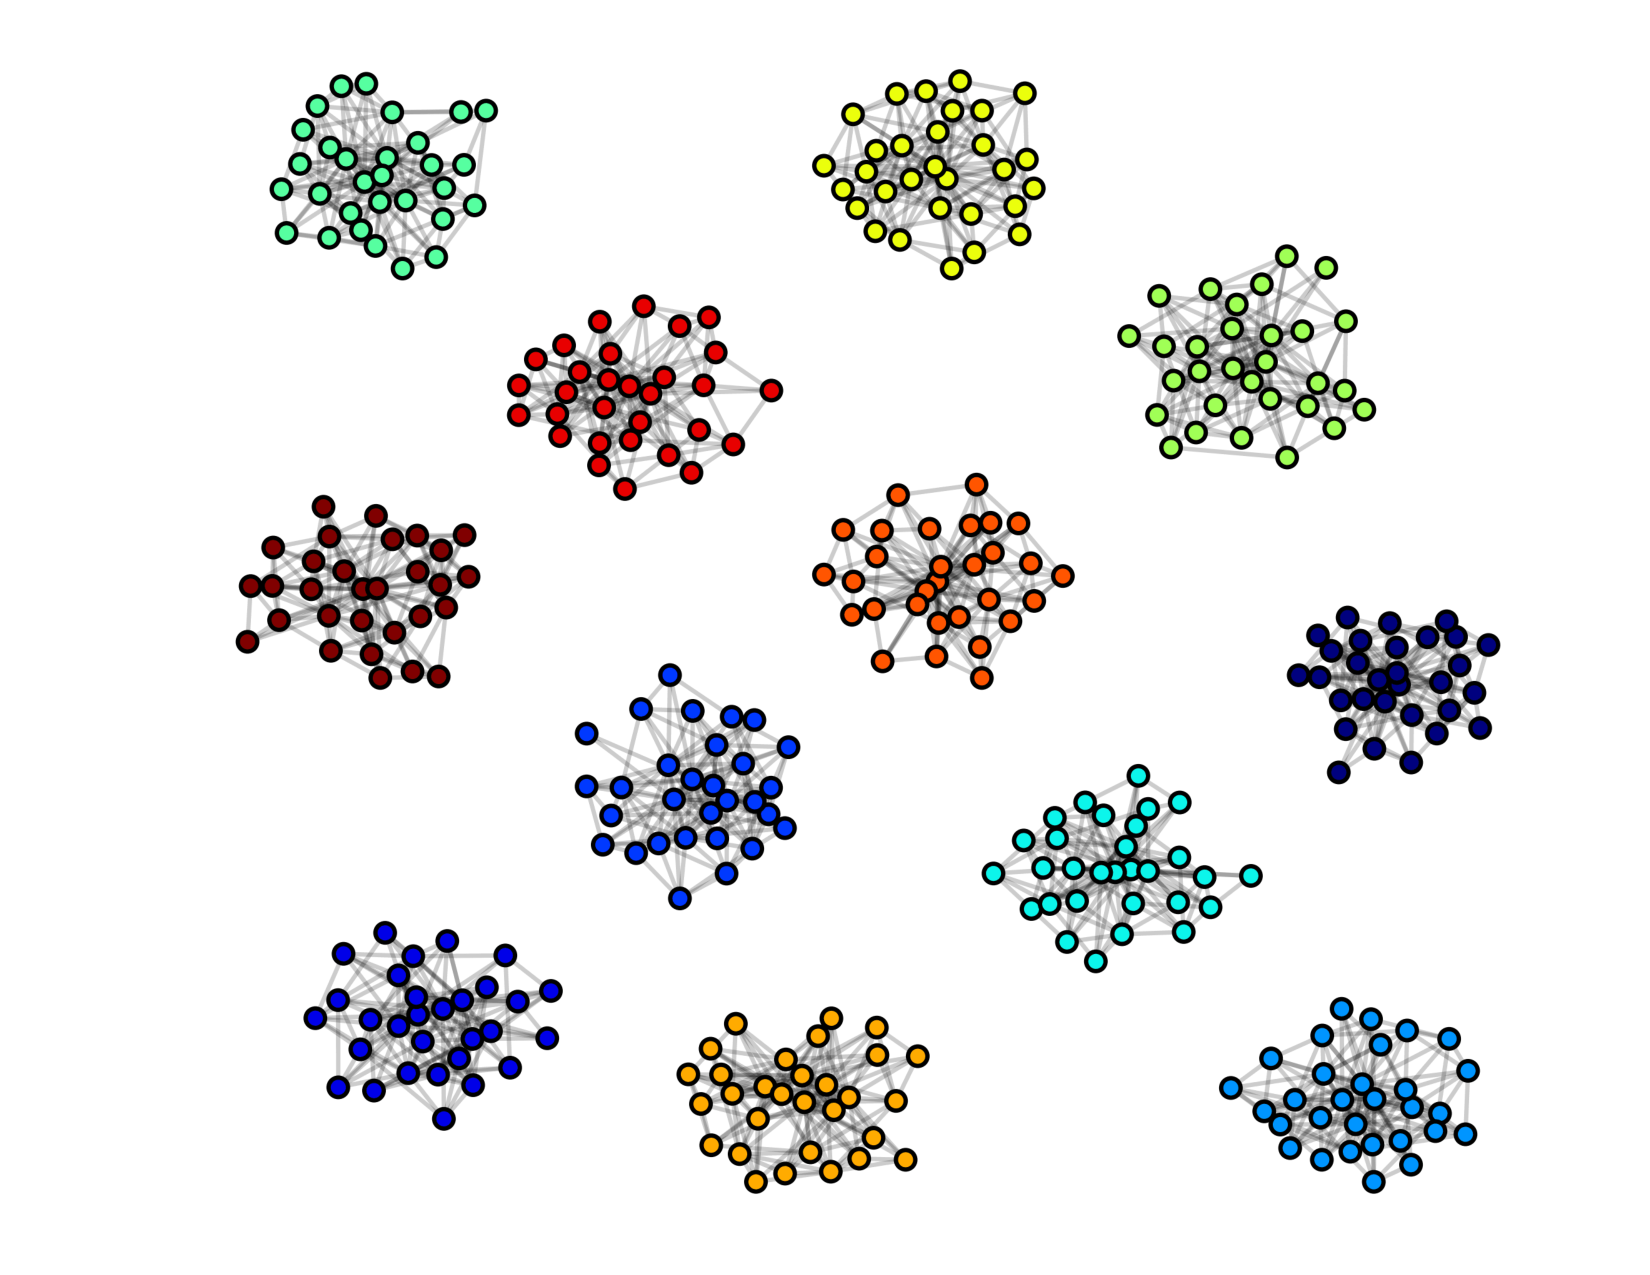
\includegraphics[scale=0.22]{Images/datasetgen1.pdf}
		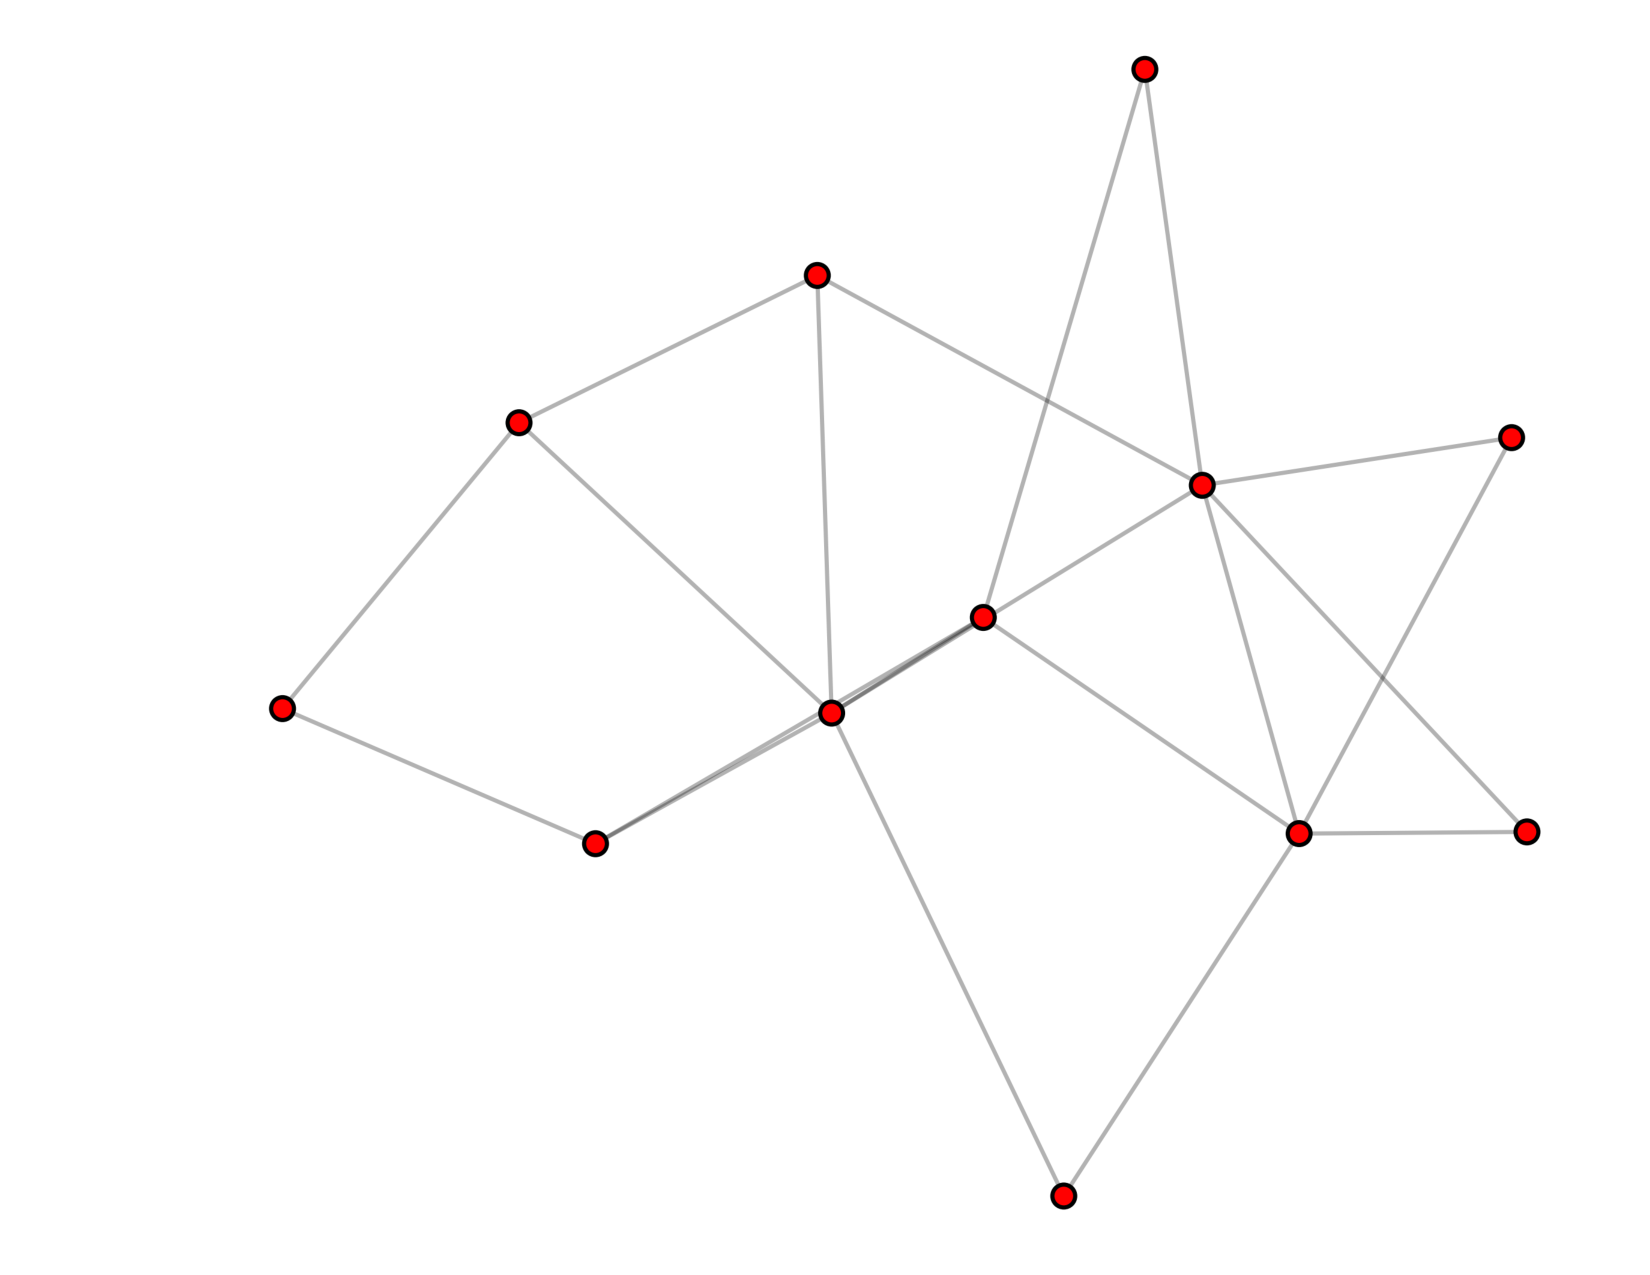
\includegraphics[scale=0.22]{Images/datasetgen2.pdf}
	\end{center}
	\item
	After the creation of small clusters like shown above, create a template shown in the \textbf{fig.2} using a powerlaw cluster graph generator with number of nodes as the number of clusters and add edges between the nodes of one cluster to another cluster from the template using reduced edge addition probabilities (shown in \textbf{fig.3}).
	\begin{center}
		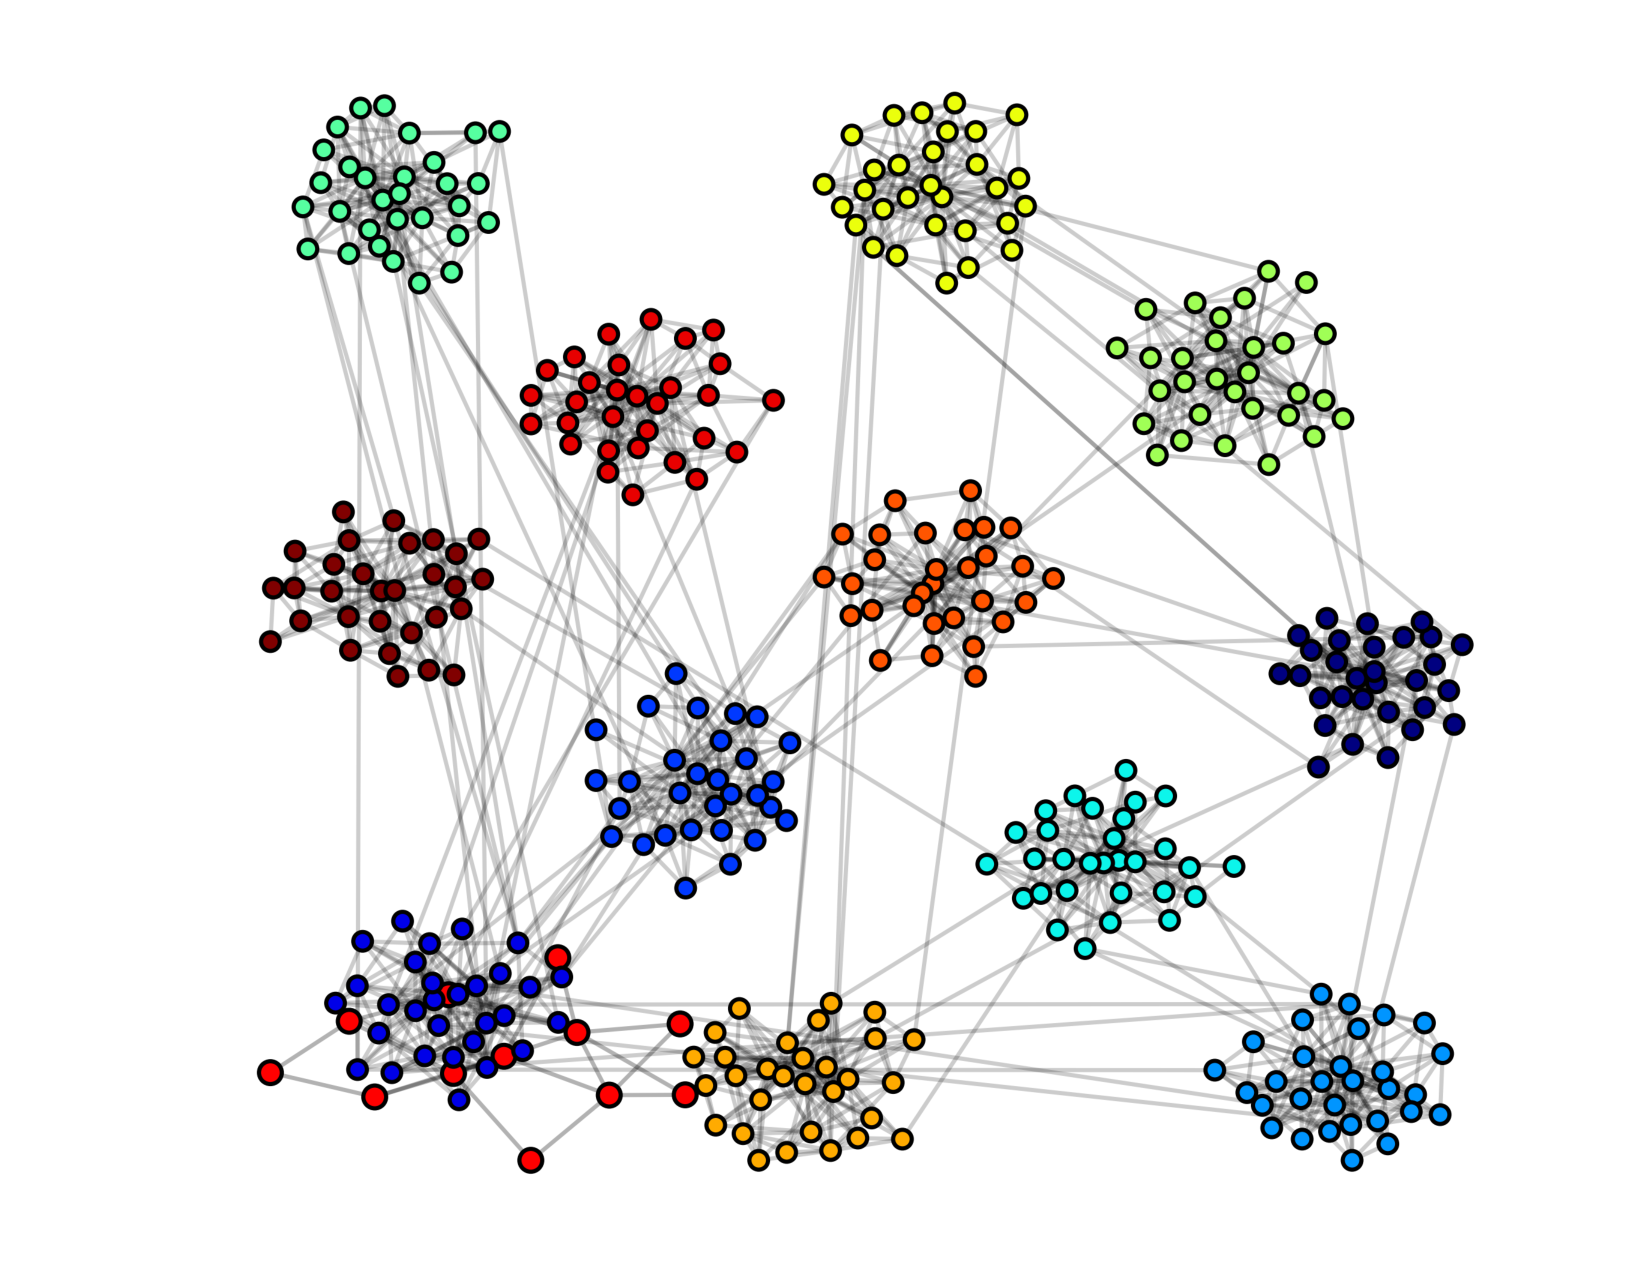
\includegraphics[scale=0.22]{Images/datasetgen3.pdf}
		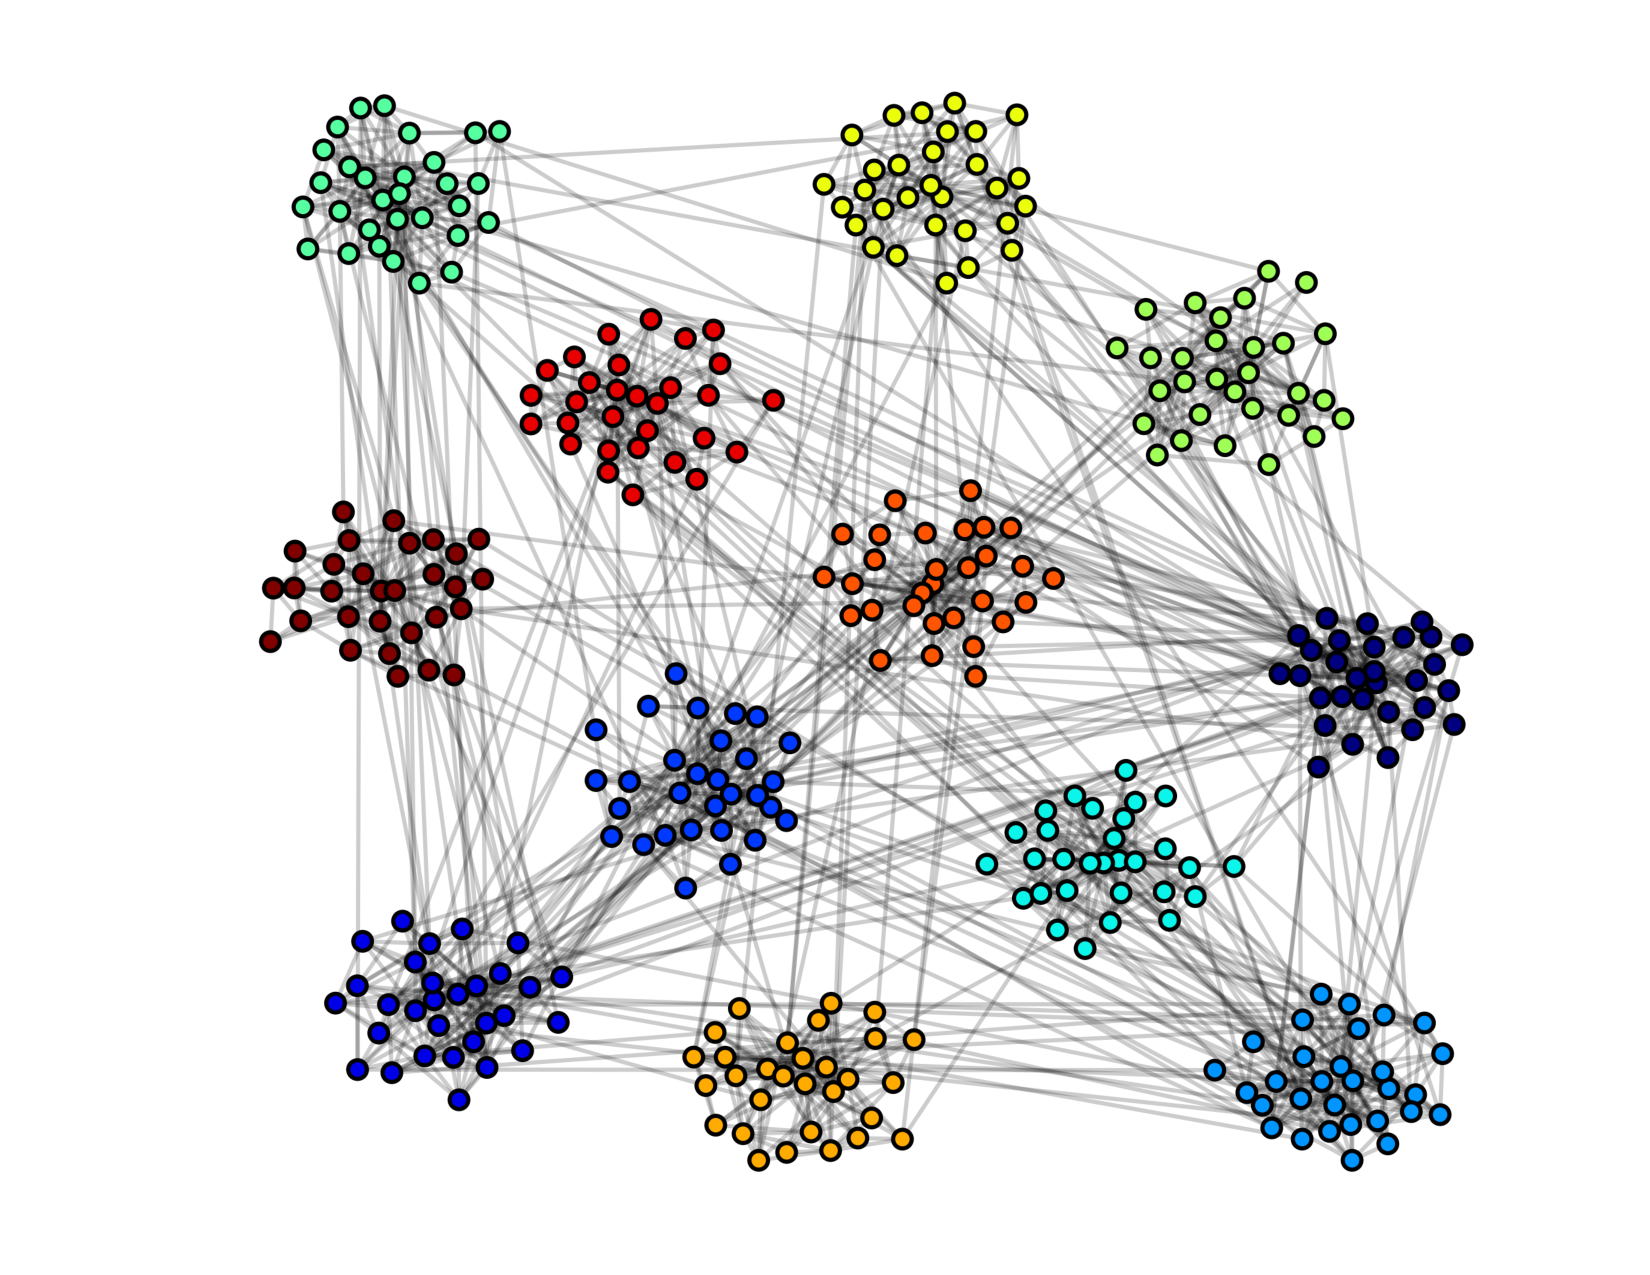
\includegraphics[scale=0.22]{Images/datasetgen4.pdf}
	\end{center}
	\item
	Repeat the above step by generating random templates and random edge addition probabilities until the graph becomes a social network.
\end{enumerate}
%!Tex root = Report.tex
\Section{Agglomerative Clustering}
Agglomerative Clustering \cite{agglo} is a method of cluster analysis which seeks to build a hierarchy of clusters from "bottom-up" approach. In this approach, each node in the graph starts with a cluster of its own and pairs of clusters are merged as one moves up the hierarchy. In order to decide which clusters should be combined, a measure of similarity between sets of clusters is required. Two measures are used in our work to combine single node clusters and multi-node clusters:
\SubSection{Structural Similarity Index}
Let $ G = (V,E,w) $ be a weighted undirected network and $ w(e) $ be the weight of the edge $ e $. For a node $ u \in V $, we define $ w(\{u,u\}) = 1 $. The structure neighborhood of a node $ u $ is the set $ \Gamma(u) $ containing $ u $ and its adjacent nodes which are incident with a common edge with $ u : \Gamma(u) = \{v \in V|\{u,v\} \in E\} \bigcup \{u\}$. The structural similarity \cite{shrink} between two adjacent nodes $ u $ and $ v $ is then
	
	$$\large \sigma (u,v) = \frac{\sum_{x \epsilon \in (u)\cap \in (v)} w(u,x).w(v,x))}{\sqrt{\sum_{x\epsilon \in (u)}w^2(u,x)}\sqrt{\sum_{x\epsilon \in (v)}w^2(v,x)}}$$
	
	The above structural similarity index can be replaced by other similarity definitions such as Jaccard similarity. Our internal testing results showed that the structural similarity index is better.

\SubSection{Clustering Coefficient}
Clustering coefficient \cite{clustcoeff} is a measure of degree to which nodes in a graph tend to cluster together. Our study of social network graphs suggested that nodes in communities with higher clustering coefficient tend to have high edges per node and are tightly connected.\\
	Let $ G = (V,E,w)$ be a graph consists of a set of vertices $ V $ and set of edges $ E $ between them. An edge $ e_{ij} $ connects vertex $ v_i $ with vertex $ v_j $. The neighborhood $ N_i $ for a vertex $ v_i $ is defined as its immediately connected neighbors as follows: 
	$$ N_i = \{ v_j: e_{ij} \in E \wedge e_{ij} \in E \}$$
	The local clustering coefficient $ C_i $ for a vertex $ v_i $ is then given by the proportion of links between the vertices within its neighborhood divided by the number of links that could possibly exist between them. An undirected graph has the property that $ e_ij $ and $ e_ji $ are considered identical. Therefore, if a vertex $ v_i $ has $ k_i $ neighbors then $ k_i(k_i - 1)/2 $ edges could exist among the vertices within the neighborhood. Therefore, local clustering coefficient for directed graphs: 
		$$\large C_i = \frac{2|{e_{jk}:v_j, v_k \epsilon N_i, e_{jk} \epsilon E}|}{k_i(k_i-1)}$$
	and clustering coefficient for the whole network is given as the average of the local clustering coefficients of all the vertices $ n $:
0		$$ C = \frac{1}{n} \sum_{i=1}^{n} C_i$$


\Section{Implementation}
Clustering algorithm is implemented in python using two pass approach and has two separate interfaces for Neo4j \cite{neo4j} and GraphLab \cite{graphlab} for querying node information. Each pass is described below.
\begin{itemize}
	\item
	\textbf{First pass}: Start breadth first search with 20 randomly sampled nodes from the database. Request neighbor list of each node using queries provided by Neo4j and Graphlab. As we get neighbor list of a node, calculate structural similarity index of the node with respect to already processed nodes and if similarity index is more than a tuned value of index threshold, combine the nodes into a cluster. This is repeated with each node as soon as we get its neighbor list. Query used for requesting neighbor list:
		\begin{itemize}
			\item
			Neo4j:
			\begin{verbatim}
			START b = node:community('id:given\_node') MATCH b-[:KNOWS]-a return a
			\end{verbatim}
			The index \texttt{community} is created on nodes during data insertion phase.
			\item
			GraphLab: 
			\begin{verbatim}
			graph = graphlab.Graph()
			neighbor_list = graph.get_edges(src_ids=[str(nodeId)])
			\end{verbatim}
		\end{itemize}
	\item
	\textbf{Second pass}: At the end of the first pass, we see a list of clusters generated using structural similarity index calculations explained above. To begin with, sort the list of clusters with respect to the number of nodes in the group from large to small clusters. Iteratively pick up the clusters with smallest size (i.e. one at the end of the cluster list) and try to combine it with the (large) clusters on the top of the list. For each pair of clusters, clustering coefficient ($ C_{ij} $) of the combination of clusters is calculated and compared it with the clustering coefficient of individual clusters. When $ C_{ij} $ is greater than a tune factor ($ k $) of $ C_i $ and $ C_j $, clusters are merged into one, i.e. 
	\begin{center}
		$ C_{ij} > kC_i$ and $C_{ij} > kC_j $.
	\end{center} 
	This process is repeated until there are no more clusters that can be merged.
\end{itemize}

%!Tex root = Report.tex
\Section{Evaluation}
\SubSection{Datasets}
As mentioned before datasets are generated using \texttt{networkx} library and there are two types of datasets, one sparse and two dense. Sparsity is measured based on the clustering coefficient of the graphg. Sparse random graphs have a small clustering coefficient while the dense graphs have large clustering coefficient.\\
\\
We have created six groups of datasets each with two graph datasets with a fixed number of edges. One graph is a sparse graph while the other one is dense. Below is the table of all the datasets generated for testing.
\begin{table}[h]
\centering
	\begin{tabular}{|r|r|r|r|}
		\hline
		\multicolumn{1}{|c|}{Dataset} & \multicolumn{1}{c|}{Total Edges} & \multicolumn{1}{c|}{Dense (nodes)} & \multicolumn{1}{c|}{Sparse(nodes)} \\ \hline
		1                             & 20,000                           & 900                                & 2,000                              \\ \hline
		2                             & 50,000                           & 2,100                              & 5,000                              \\ \hline
		3                             & 100,000                          & 4,000                              & 9,500                              \\ \hline
		4                             & 200,000                          & 8,000                              & 19,000                             \\ \hline
		5                             & 500,000                          & 20,000                             & 47,000                             \\ \hline
		6                             & 1,000,000                        & 40,000                             & 91,000                             \\ \hline
	\end{tabular}
\end{table}
The following graph shows the distribution of nodes with respect to their degree for each node\\
?? include a graph of the ??
\SubSection{Setup}
The following are the set of machines used for testing. 
\begin{itemize}
	\item
	Neo4j: Amazon EC2 instance with 2 vCPUs and 7.5GB memory with 20GB disk space.
	\item
	GraphLab: Amazon EC2 instance with 4 vCPUs and 7.5GB memory with 20GB disk space.
\end{itemize}
\SubSection{Testing and measurements}
\begin{enumerate}
	\item
	\textbf{Execution time:} All the above datasets are run on both Neo4j and GraphLab systems. Time of execution is calculated starting from the beginning of the clustering algorithm till the end. Execution time does not include the time taken for the dataset to load into the database systems. On an another note, GraphLab is a graph processing system which loads the dataset into memory and is really quick, for example, a dataset of 100,000 edges takes around half a second to load into memory, whereas Neo4j stores each node in its database on a persistent storage.
\end{enumerate}
%!Tex root = Report.tex
\Section{Results}
\SubSection{Performance}
This section presents results of performance comparison between Neo4j and GraphLab. 
\begin{itemize}
\item Figure \ref{fig:dense-edges} and \ref{fig:sparse-edges} show the comparison between Neo4j and GraphLab with varying number of edges in the dataset. GraphLab performs better than Neo4j over the entire range of dataset generated.
\item Similar comparison with the number of nodes per dataset is shown in plots \ref{fig:dense-nodes} and \ref{fig:sparse-nodes}. Over the small dataset, the relative difference between GraphLab and Neo4j is high, however it reduces as the data scales up.
\item Figure \ref{fig:neo4j-sparse-dense} and \ref{fig:graphlab-sparse-dense} show that the execution time for a sparse dataset is always smaller than dense datasets. This is expected because dense graphs have high number of neighbors which lead to higher query processing time.
\end{itemize}
\SubSection{Cluster Purity}
This section introduces one of the external criteria of clustering quality. Purity is a simple and transparent evaluation measure. To compute purity, each cluster is assigned to the class which is most frequent in the cluster, and then the accuracy of this assignment is measured by counting the number of correctly assigned documents and dividing by N. Here, class is the set of clusters we already know in the synthetic input data for clustering and N is the total number of nodes in the graph. Formally
\begin{equation}
purity(\Omega, C ) = \frac{1}{N}\sum_{k} max_{j}|w_{k} \bigcap c_{j}|
\end{equation}
where $\Omega = \{w_{1}, w_{2},....,w_{k}\}$ is the set of clusters and $C=\{c_{1},c_{2},...,c{j}\}$ is the set of classes.
High purity is easy to achieve when the number of clusters is large - in particular, purity is 1 if each document gets its own cluster. However, we are getting number of resulting clusters almost equal to the number of gold standard clusters. Hence this measure is reasonable here to judge performance of our clustering algorithm.\\
\textbf{NOTE:} We know the number of actual clusters in the synthetic data generated from networkx. Therefore we will call it as gold standard data.

\begin{itemize}
\item Performance of our implementation is better on dense graph as compared to sparse graph, which is expected considering nodes are scattered in sparse graph.
\item Average clustering purity for dense graph having number of edges $> 200,000$ is $0.92$.
\item Average clustering purity for sparse graph having number of edges $> 200,000$ is $0.84$.
\item For smaller datasets having edge counts between $20,000$ to $100,000$, we are achieving nearly perfect clustering. Clustering coefficient for them is $>0.98$ with same number of clusters/ classes in output as in the gold data.
\end{itemize}

	\begin{figure}
		\begin{minipage}{.5\textwidth}
			\centering
			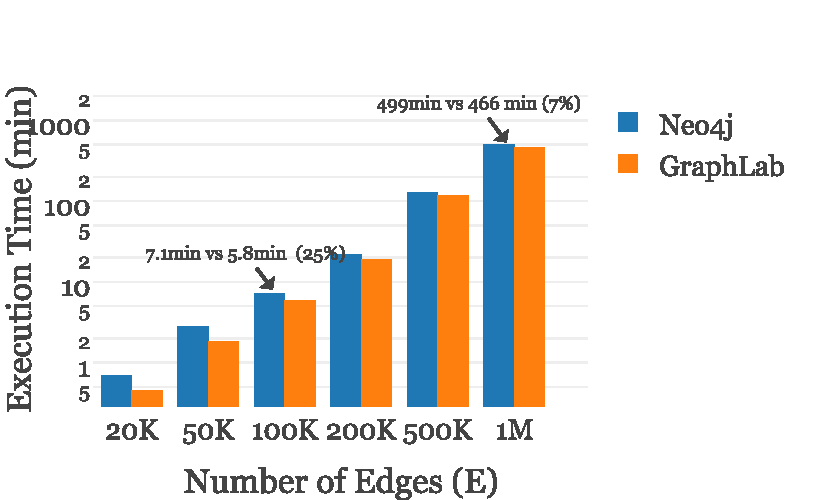
\includegraphics[scale=0.5]{Graphs/dense-edges.pdf}
			\caption{Dense datasets - Neo4j vs GraphLab\label{fig:dense-edges}}
		\end{minipage}
		\begin{minipage}{.5\textwidth}
			\centering
			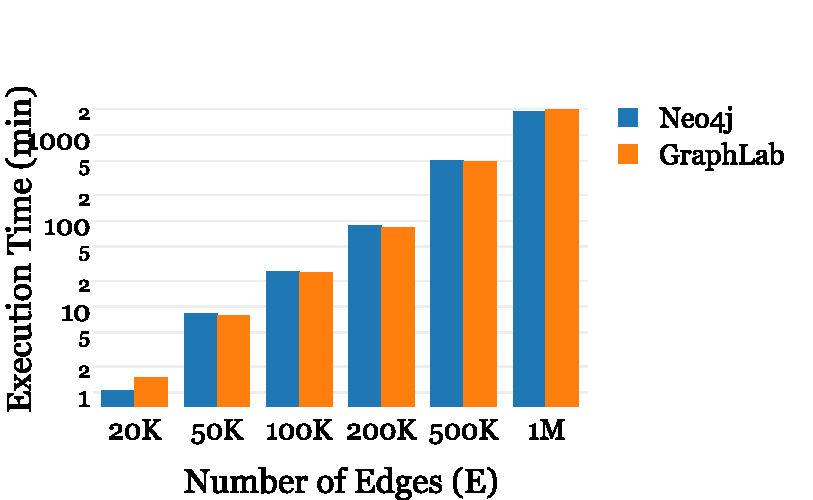
\includegraphics[scale=0.5]{Graphs/sparse-edges.pdf}
			\caption{Sparse datasets - Neo4j vs GraphLab\label{fig:sparse-edges}}
		\end{minipage}
	\end{figure}
	
	
	\begin{figure}
		\begin{minipage}{.5\textwidth}
			\centering
			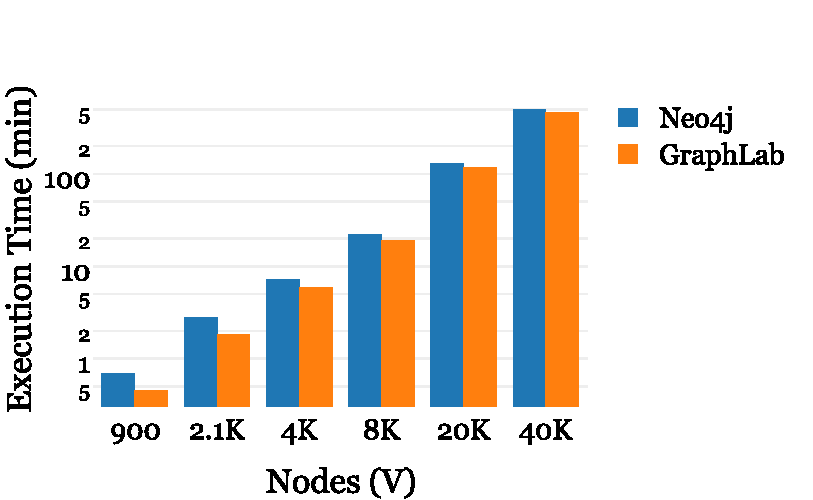
\includegraphics[scale=0.5]{Graphs/dense-nodes.pdf}
			\caption{Dense datasets - Neo4j vs GraphLab\label{fig:dense-nodes}}
		\end{minipage}
		\begin{minipage}{.5\textwidth}
			\centering
			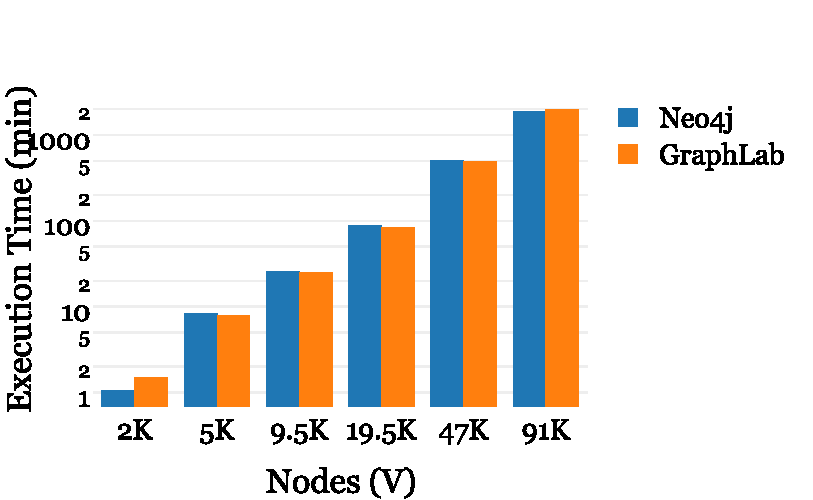
\includegraphics[scale=0.5]{Graphs/sparse-nodes.pdf}
			\caption{Sparse datasets - Neo4j vs GraphLab\label{fig:sparse-nodes}}
		\end{minipage}
	\end{figure}
	
	\begin{figure}
		\begin{minipage}{.5\textwidth}
			\centering
			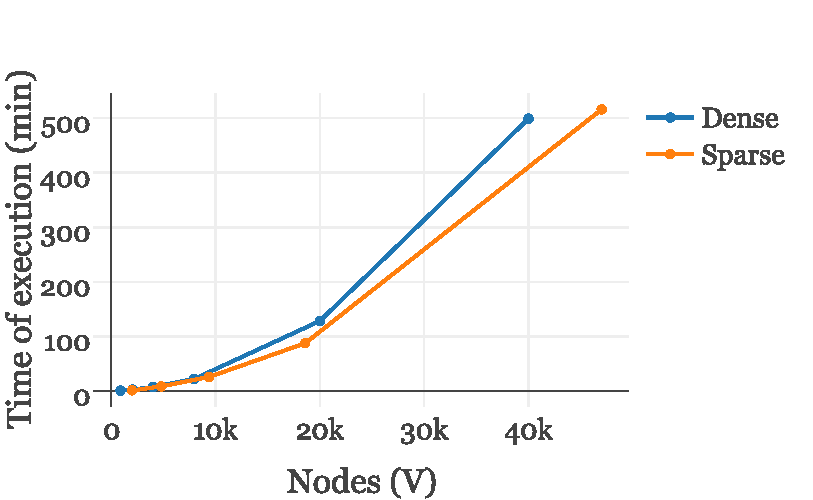
\includegraphics[scale=0.5]{Graphs/neo4j-sparse-dense.pdf}
			\caption{Neo4j - Dense vs Sparse datasets\label{fig:neo4j-sparse-dense}}
		\end{minipage}
		\begin{minipage}{.5\textwidth}
			\centering
			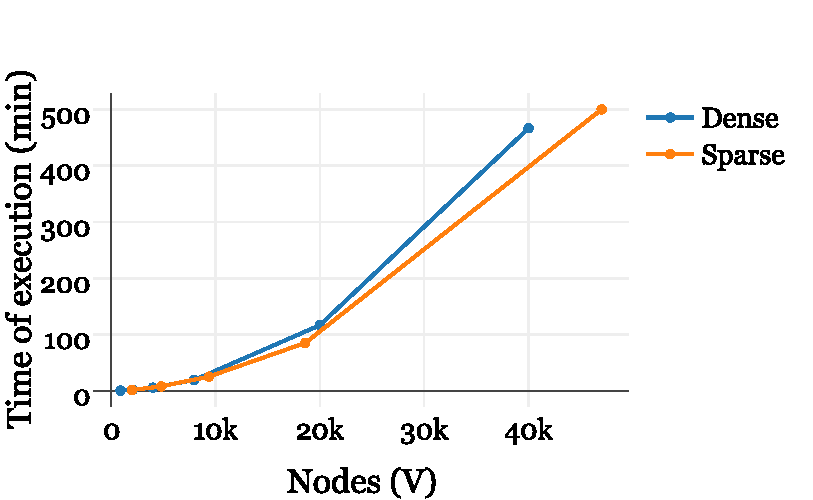
\includegraphics[scale=0.5]{Graphs/graphlab-sparse-dense.pdf}
			\caption{GraphLab - Dense vs Sparse datasets\label{fig:graphlab-sparse-dense}}
		\end{minipage}
	\end{figure}
	

\SubSection{Clustering on real world dataset: Facebook}
This section presents clustering performance of real world social network Facebook \cite{facebookdata} from Stanford Large Network Dataset Collection \cite{snap}.\\
\\
\textbf{Facebook Dataset Details:}
\begin{itemize}
	\item
	Nodes: 4039
	\item
	Edges: 88234
	\item
	Average clustering coefficient:	0.6055
	\item
	Number of triangles:	1612010
\end{itemize}
\noindent
\textbf{Facebook Dataset Results:}
\begin{itemize}
	\item
	Total number of clusters detected: 8
	\item
	Total Execution Time (Neo4j): 11.3 minutes
	\item
	Total Execution Time (GraphLab): 9.5 minutes
	\item
	List of clusters with number of nodes in them:\\
	Cluster-1 Nodes:1368\\
	Cluster-2 Nodes:770\\
	Cluster-3 Nodes:753\\
	Cluster-4 Nodes:590\\
	Cluster-5 Nodes:316\\
	Cluster-6 Nodes:211\\
	Cluster-7 Nodes:21\\
	Cluster-8 Nodes:10	
\end{itemize}
\begin{figure}
	\centering
	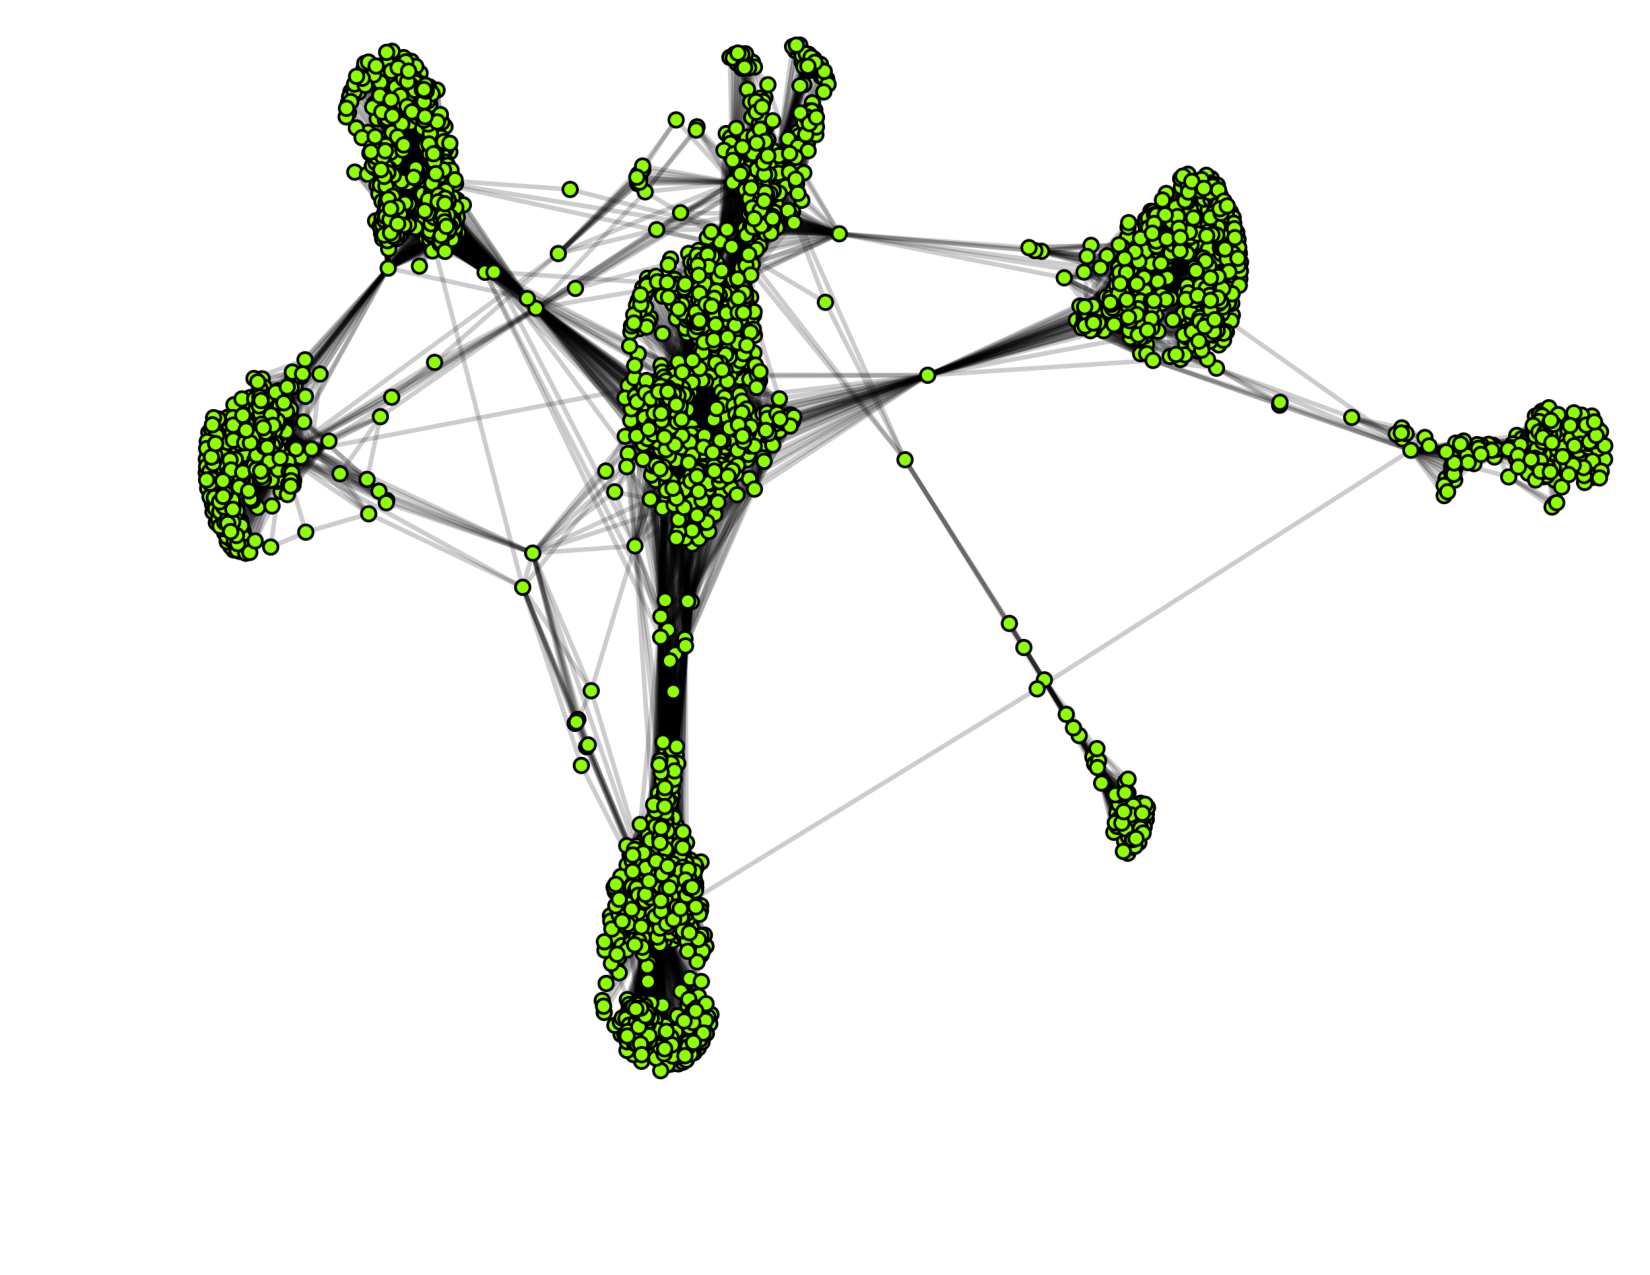
\includegraphics[scale=0.4, trim=0 0 20 0]{Images/before_facebook.pdf}
	\caption{Facebook Dataset - Before Clustering\label{fig:fb-before}}
\end{figure}
\begin{figure}
	\centering
	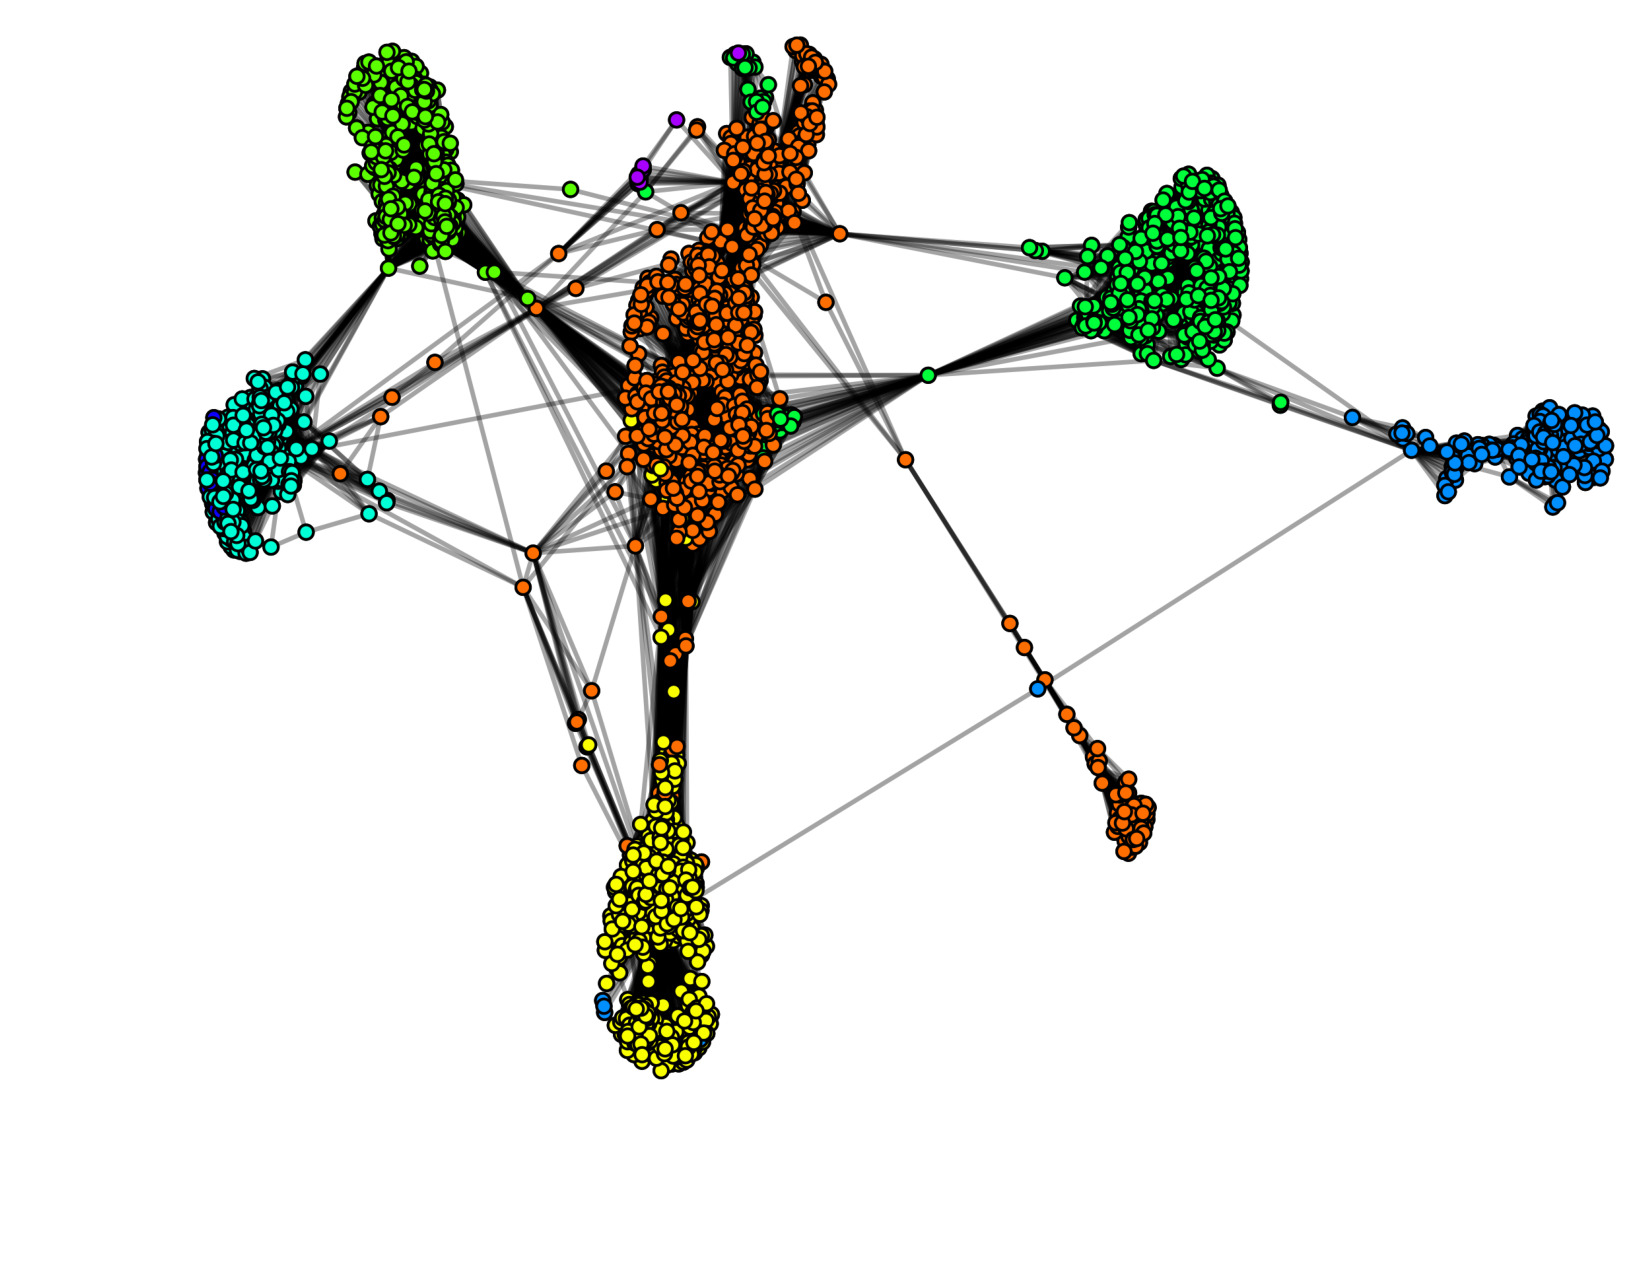
\includegraphics[scale=0.4, trim=0 0 20 0]{Images/after_facebook.pdf}
	\caption{Facebook Dataset - After Clustering (Neo4j/GraphLab)\label{fig:fb-after}}
\end{figure}

%\Section{References}
%Some citation ~\cite{IEEEhowto:kopka}


% use section* for acknowledgement
%\section*{Acknowledgment}


%The authors would like to thank...
%more thanks here

\begin{thebibliography}{1}
\small
%\bibitem{IEEEhowto:kopka}
%H.~Kopka and P.~W. Daly, \emph{A Guide to \LaTeX}, 3rd~ed.\hskip 1em plus
%  0.5em minus 0.4em\relax Harlow, England: Addison-Wesley, 1999.
\bibitem{WillHerb} William H. E. Day, Herbert Edelsbrunner "Efficient algorithms for agglomerative hierarchical clustering methods".
\bibitem{Chris}Chris Fraley "Algorithms for model-based Gaussian hierarchical clustering".
\bibitem{CFO}[3] CF Olson "Parallel algorithms for hierarchical clustering".
\bibitem{SteinKar}M Steinbach, G Karypis, V Kumar "A comparison of document clustering techniques".
\bibitem{ZhaoKar}Y Zhao, G Karypis "Evaluation of hierarchical clustering algorithms for document
datasets".
\bibitem{GuhaRat}S Guha, R Rastogi, K Shim "CURE: an efficient clustering algorithm for large databases".
\bibitem{McAuLesk}J. McAuley and J. Leskovec. "Learning to Discover Social Circles in Ego Networks".
\bibitem{benchmark}http://istc-bigdata.org/index.php/benchmarking-graph-databases.
\bibitem{snap} http://snap.stanford.edu/data/.
\bibitem{MishraSchrei}N. Mishra, R. Schreiber, I. Stanton, R. Tarjan “Clustering Social Networks”.
\bibitem{Held}P.Held, K.Dannies “Clustering on Dynamic Social Network Data”.

\end{thebibliography}

\end{document}


